Le projet sera géré selon la méthodologie \textbf{Scrum}, favorisant une approche agile avec des cycles itératifs appelés \textbf{sprints}. Le \textbf{Product Owner}, l’\textbf{équipe de développement} et le \textbf{Scrum Master} collaboreront pour assurer une livraison progressive des fonctionnalités clés.

\subsection*{Acteurs Scrum et Missions}
\begin{longtable}{|m{3cm}|m{8cm}|m{2cm}|}
\hline
\textbf{Rôle} & \textbf{Mission} & \textbf{Acteur} \\
\hline
\endfirsthead
\hline
\textbf{Rôle} & \textbf{Mission} & \textbf{Acteur} \\
\hline
\endhead
% \hline
\endfoot
Product Owner & 
- Définir et prioriser les fonctionnalités du produit (Product Backlog). \newline
- Assurer que l'équipe travaille sur les fonctionnalités les plus importantes. \newline
- Valider les livrables à la fin de chaque sprint. &
Pr Ammeri Charfeddine \\
\hline
Équipe de Développement & 
- Concevoir, développer et tester les fonctionnalités du produit. \newline
- Participer aux réunions de planification et de revue de sprint. \newline
- Assurer la qualité du code et des livrables. &
Zaibi Racha \\
\hline
Scrum Master & 
- Faciliter les réunions Scrum (Daily Stand-up, Sprint Planning, Sprint Review, Retrospective). \newline
- Supprimer les obstacles qui empêchent l'équipe de progresser. \newline
- Assurer que l'équipe suit les principes Scrum. &
Ouni Ghada\\
\hline
\caption{Acteurs du projet} 
\end{longtable}

\subsection*{Organisation du Backlog}
Le \textbf{Product Backlog} regroupe l’ensemble des fonctionnalités à développer pour le système. Chacune est formulée sous forme de \textit{User Story}, garantissant une approche centrée sur l’utilisateur.

Chaque fonctionnalité sera développée et livrée en plusieurs \textbf{sprints}, selon les priorités établies par le \textit{Product Owner}. Elles sont classées selon la méthode \textbf{MoSCoW}, qui définit les niveaux de priorité pour chaque tâche.

\section*{Backlog du Projet}
% Le \textbf{Backlog} est un élément central de la méthodologie \textbf{Scrum}. Il regroupe toutes les spécifications fonctionnelles et techniques du produit.

\begin{longtable}{|c|p{9cm}|c|}
    \hline
    \textbf{ID} & \textbf{Tâche} & \textbf{Priority} \\
    \hline
    \endfirsthead
    \hline
    \textbf{ID} & \textbf{Tâche} & \textbf{Priority} \\
    \hline
    \endhead
    % \hline
    \endfoot
    M-01 & Collecte des données en temps réel à partir des moniteurs Mindray via API/HL7. & M \\
    \hline
    M-02 & Détection et reconnaissance des valeurs vitales via OCR pour les machines anciennes. & M \\
    \hline
    M-03 & Génération et gestion des alertes en fonction des seuils prédéfinis. & M \\
    \hline
    M-04 & Envoi d’alertes aux médecins et infirmiers via notifications push (FCM) et e-mail. & M \\
    \hline
    M-05 & Interface web et mobile pour visualiser les données des patients et gérer les alertes. & M \\
    \hline
    M-06 & Authentification et gestion des utilisateurs (médecins, infirmiers, administrateurs). & M \\
    \hline
    M-07 & Stockage et historique des données pour analyse et suivi. & M \\
    \hline
    M-08 & Conformité aux réglementations médicales (sécurité des données, chiffrement). & M \\
    \hline
    M-09 & Tests de validation de la collecte de données (comparaison entre API et OCR). & M \\
    \hline
    S-01 & Intégration avec d’autres modèles de moniteurs (Edan, etc.). & S \\
    \hline
    S-02 & Configuration des seuils d’alerte personnalisés par patient ou par bloc. & S \\
    \hline
    S-03 & Gestion des horaires de filtrage des alertes pour le personnel médical. & S \\
    \hline
    S-04 & Interface d’administration pour configurer les seuils d’alerte et gérer les utilisateurs. & S \\
    \hline
    S-05 & Notifications SMS en plus des notifications push et e-mail. & S \\
    \hline
    S-06 & Scalabilité du système pour gérer un nombre croissant de patients et d’appareils. & S \\
    \hline
    C-01 & Intégration avec des systèmes tiers (IQ Messenger SmartApp, Xchart.com). & C \\
    \hline
    C-02 & Analyse prédictive des données pour anticiper les alertes critiques. & C \\
    \hline
    C-03 & Interface mobile avancée avec des graphiques interactifs pour les données des patients. & C \\
    \hline
    C-04 & Support multilingue pour l’interface utilisateur. & C \\
    \hline
    C-05 & Gestion des alertes par priorité (critique, moyen, faible). & C \\
    \hline
    C-06 & Historique des alertes avec possibilité de filtrage par date, patient, ou type d’alerte. & C \\
    \hline
    % W-01 & Intégration avec des systèmes de gestion hospitalière (HIS) tiers. &W \\
    % \hline
    % W-02 & Déploiement du système dans plusieurs hôpitaux ou centres médicaux. &W \\
    % \hline
    % W-03 & Analyse avancée des données avec intelligence artificielle pour le diagnostic médical. &W \\
    % \hline
    % W-04 & Support pour d’autres langues de programmation ou frameworks non prévus initialement. &W \\
    % \hline
    % W-05 & Développement d’une application desktop en plus des interfaces web et mobile. &W \\
    % \hline
\caption{Backlog du Projet avec Priorités MoSCoW} 
\end{longtable}
\section*{Clé des Priorités MoSCoW}
\begin{itemize}
    \item \textbf{M (Must)} : Tâches critiques nécessaires au bon fonctionnement du système.
    \item \textbf{S (Should)} : Tâches importantes qui apportent une valeur significative mais ne sont pas essentielles pour la première version.
    \item \textbf{C (Could)} : Fonctionnalités optionnelles pouvant être ajoutées si le temps et les ressources le permettent.
    \item \textbf{W (Won't Have)} : Tâches hors du périmètre de la phase actuelle du projet.
\end{itemize}

\subsection{Diagramme des cas d’utilisation global}
\begin{figure}[H]
    \centering
    \begin{minipage}{1\textwidth}
        \centering
        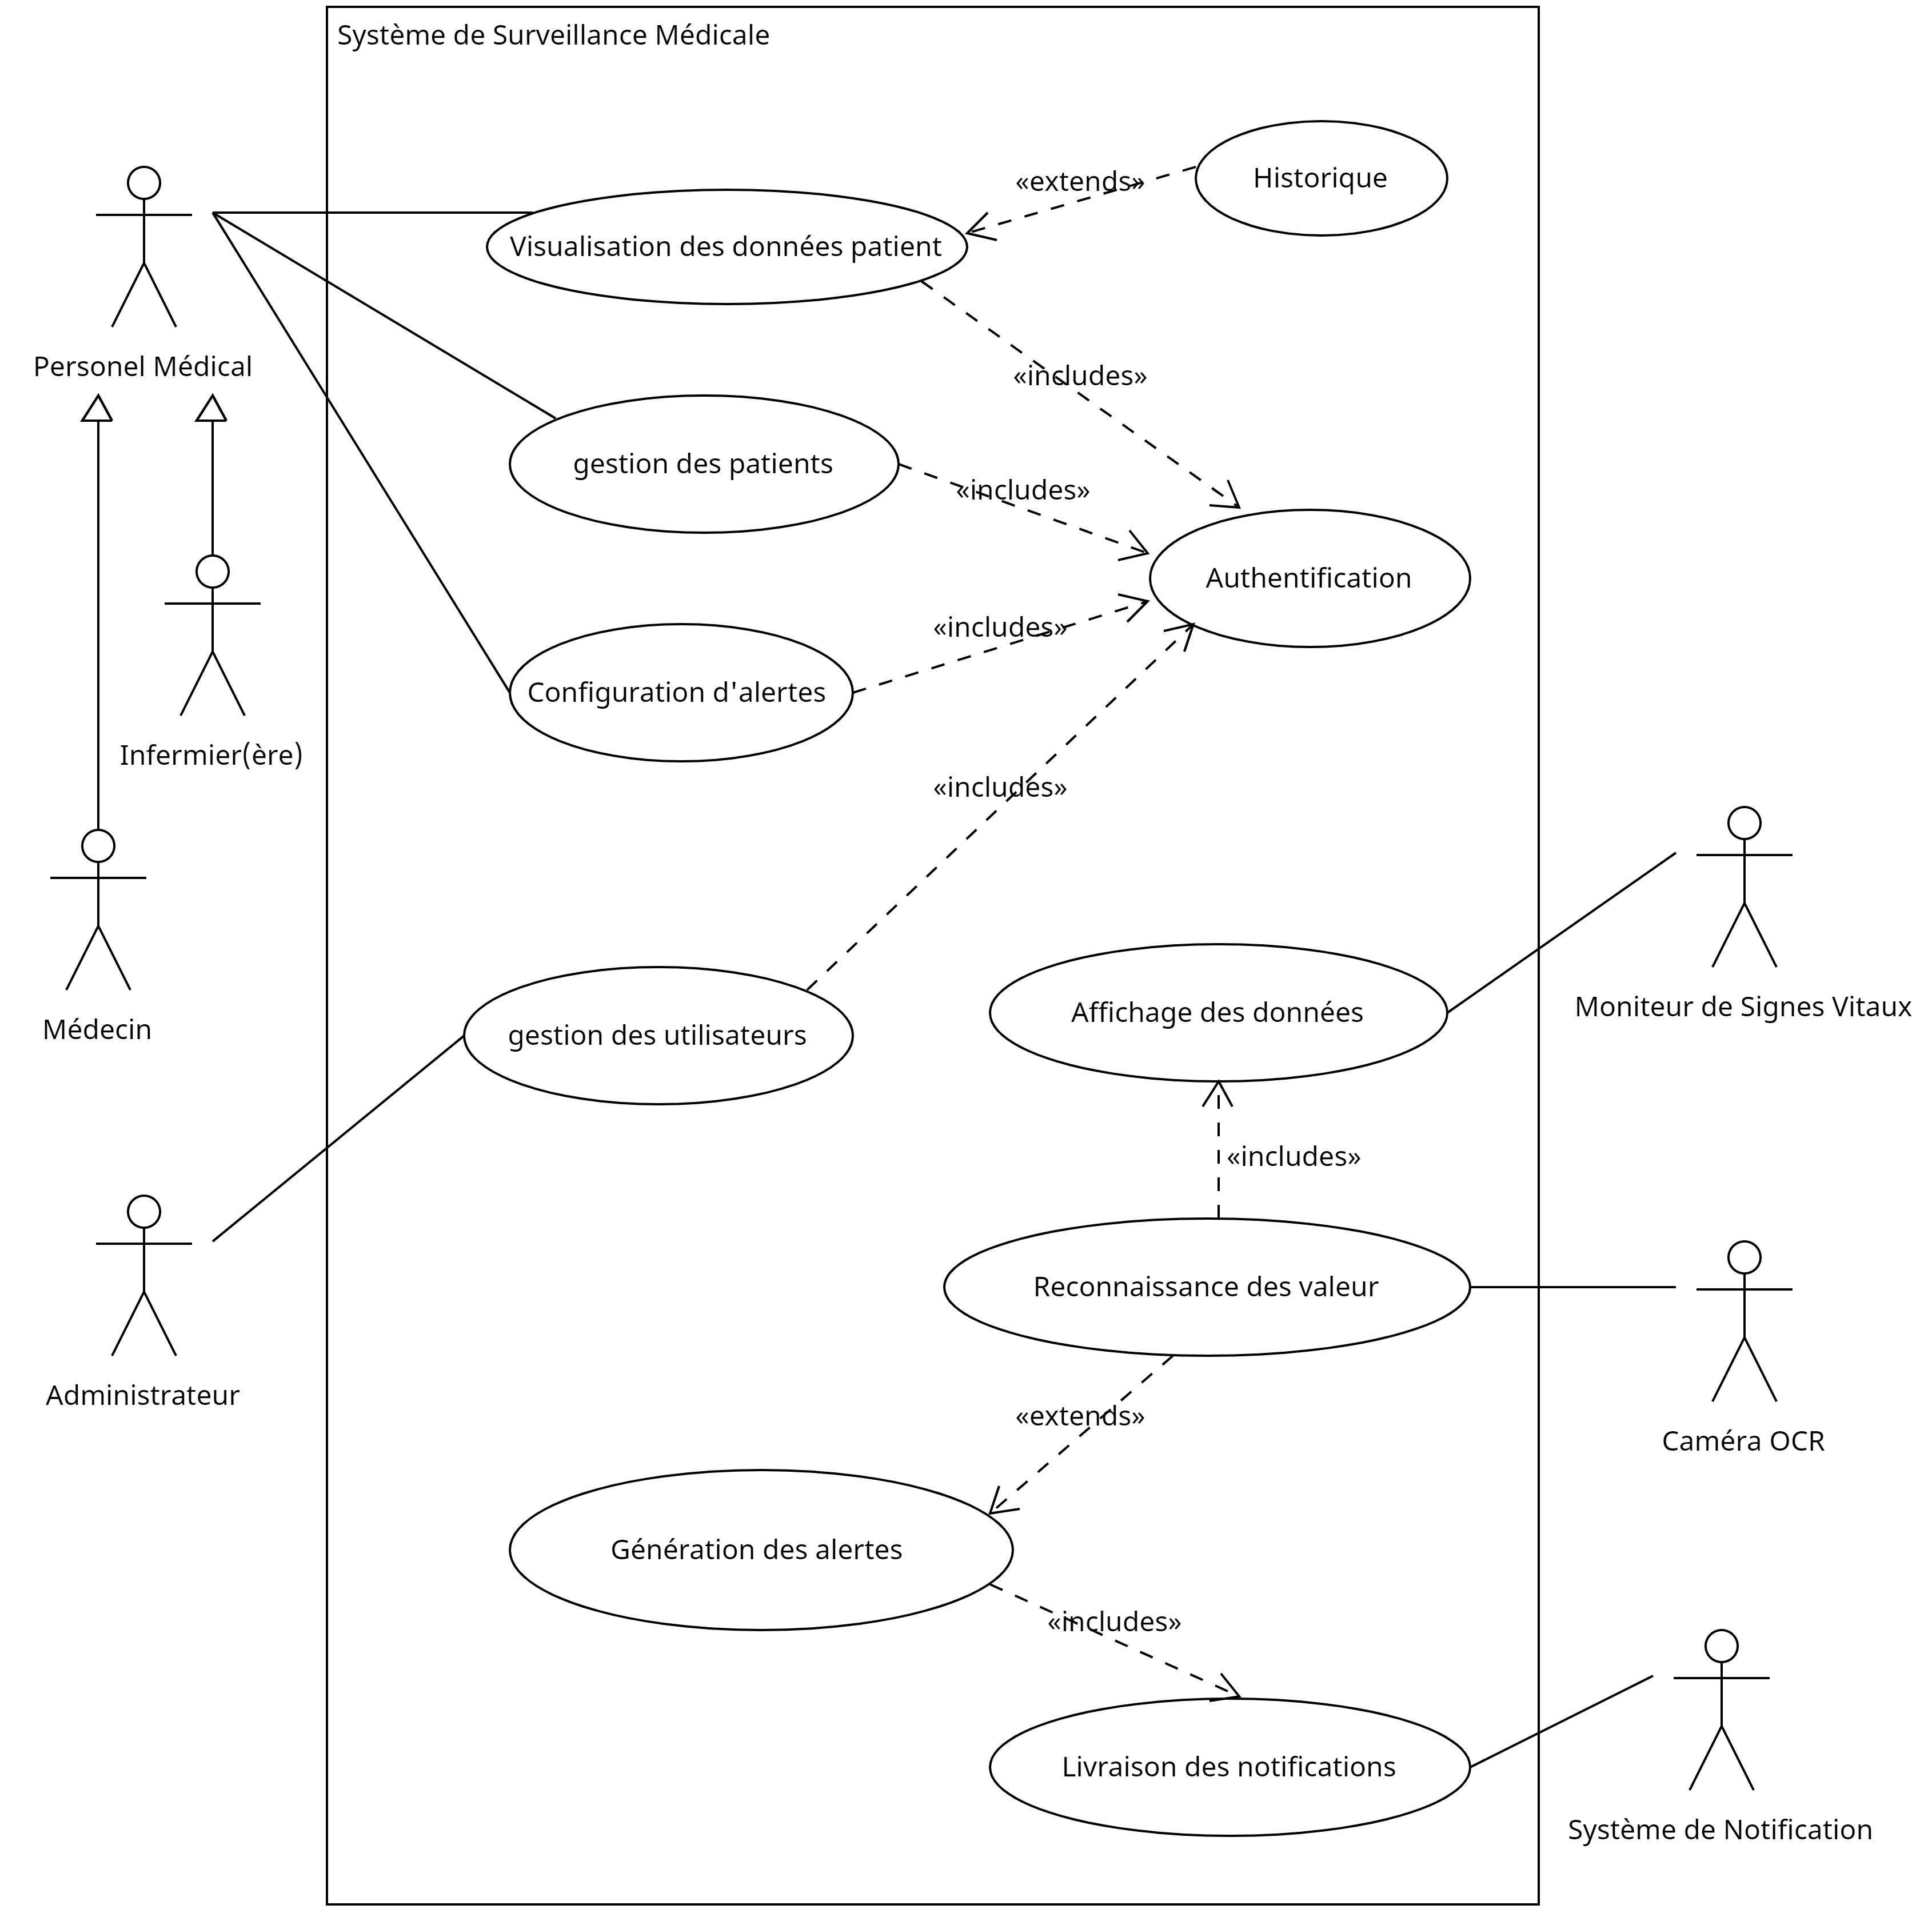
\includegraphics[width=\linewidth]{chapter2/sections/diagrams/use_case.png}
        \caption{Diagramme des cas d’utilisation global}
    \end{minipage}
\end{figure}
\subsection{Planification des sprints}
Une fois le backlog du produit finalisé, nous avons organisé la réunion de planification de sprint. L'objectif de cette réunion était de construire le backlog de sprint en se basant sur le backlog de produit défini par le Product Owner. À l'issue de cette réunion, nous avons identifié les durées prévisionnelles du travail à effectuer pour chaque sprint. Pour ce projet, nous avons divisé le travail en deux releases. La première release contient un seul sprint d'une durée de 2 semaines, tandis que la deuxième release est composée de deux sprints, chacun d'une durée de 3 semaines. La figure 2.2 illustre la répartition des sprints pour notre système.

Décrivez le plan des sprints :

\begin{itemize}
    \item \textbf{Sprint 1 : Collecte de données basée sur caméra}
    \begin{itemize}
        \item \textbf{Objectif} : Mettre en place un système de collecte de données à partir des machines anciennes en utilisant des caméras et des techniques de reconnaissance optique de caractères (OCR).
        \item \textbf{Deliverables} :
            \begin{itemize}
                \item Intégration de la caméra avec le système.
                \item Détection et extraction des valeurs vitales via OCR.
                \item Validation des données collectées par rapport aux données réelles.
            \end{itemize}
        \item \textbf{Durée} : 2 semaines.
        \item \textbf{Tâches clés} :
            \begin{itemize}
                \item Configuration des caméras et des logiciels OCR (OpenCV, Tesseract).
                \item Développement du pipeline de traitement d'images.
                \item Tests de validation des données collectées.
            \end{itemize}
        \item \textbf{Risques} : 
            \begin{itemize}
                \item Mauvaise qualité d'image affectant la précision de l'OCR.
                \item Solution : Utilisation de caméras haute résolution et prétraitement des images.
            \end{itemize}
    \end{itemize}

    \item \textbf{Sprint 2 : Collecte de données à partir des moniteurs Mindray}
    \begin{itemize}
        \item \textbf{Objectif} : Intégrer les moniteurs Mindray pour collecter des données en temps réel via des API ou des protocoles HL7.
        \item \textbf{Deliverables} :
            \begin{itemize}
                \item Connexion des moniteurs Mindray au système central.
                \item Collecte et stockage des données en temps réel.
                \item Validation de la collecte de données via API/HL7.
            \end{itemize}
        \item \textbf{Durée} : 3 semaines.
        \item \textbf{Tâches clés} :
            \begin{itemize}
                \item Configuration des API ou des protocoles HL7 pour les moniteurs Mindray.
                \item Développement du backend pour la collecte et le stockage des données.
                \item Tests de validation des données collectées.
            \end{itemize}
        \item \textbf{Dépendances} : Les données collectées via caméra (Sprint 1) doivent être validées avant de passer à ce sprint.
        \item \textbf{Risques} :
            \begin{itemize}
                \item Problèmes de compatibilité avec les API ou les protocoles HL7.
                \item Solution : Documentation technique et tests approfondis avant l'intégration.
            \end{itemize}
    \end{itemize}

    \item \textbf{Sprint 3 : Système de gestion des alertes et de notification}
    \begin{itemize}
        \item \textbf{Objectif} : Développer un système de gestion des alertes basé sur des seuils prédéfinis et envoyer des notifications au personnel médical.
        \item \textbf{Deliverables} :
            \begin{itemize}
                \item Définition des seuils d'alerte pour les valeurs vitales.
                \item Mise en place d'un système de priorisation des alertes.
                \item Intégration des mécanismes de notification (e-mail, notifications push via FCM).
            \end{itemize}
        \item \textbf{Durée} : 3 semaines.
        \item \textbf{Tâches clés} :
            \begin{itemize}
                \item Développement du module de gestion des alertes.
                \item Intégration des notifications push et e-mail.
                \item Tests de validation des alertes et des notifications.
            \end{itemize}
        \item \textbf{Dépendances} : Les données collectées dans les Sprints 1 et 2 doivent être disponibles pour ce sprint.
        \item \textbf{Risques} :
            \begin{itemize}
                \item Retards dans la livraison des alertes critiques.
                \item Solution : Optimisation du temps de réponse et tests de performance.
            \end{itemize}
    \end{itemize}
\end{itemize}

